%%%%%%%%%%%%%%%%%%%%%%%%%%%%%%%%%%%%%%%%%%%%
%LaTex template for scientific report in AGP
%%%%%%%%%%%%%%%%%%%%%%%%%%%%%%%%%%%%%%%%%%%%

\documentclass[11pt]{article}%[draft]{agujournal2019}
\usepackage{url} %this package should fix any errors with URLs in refs.
\usepackage{lineno}
\usepackage{float}
\usepackage[utf8]{inputenc}
\usepackage[margin=0.875in]{geometry}
\usepackage[inline]{trackchanges} %for better track changes. finalnew option will compile document with changes incorporated.
\usepackage{soul}
\usepackage{graphicx}
\graphicspath{ {./figures/} }

\usepackage{verbatim}
\usepackage[dvipsnames]{xcolor}
\usepackage{fancyvrb}
\usepackage[colorlinks=true,allcolors=blue]{hyperref}
\usepackage{blindtext}
\usepackage[labelfont=bf]{caption} % make figure labels bold

% redefine \VerbatimInput
\RecustomVerbatimCommand{\VerbatimInput}{VerbatimInput}%
{fontsize=0.8\footnotesize,
 %
 frame=lines,  % top and bottom rule only
 framesep=2em, % separation between frame and text
 rulecolor=\color{Gray},
 %
 label=\fbox{\color{Black}processing history of MIG-FD50-T2D},
 labelposition=topline,
 %
 commandchars=\|\(\), % escape character and argument delimiters for
                      % commands within the verbatim
 commentchar=*        % comment character
}

\usepackage[backend=bibtex,style=authoryear-icomp,maxcitenames=1,natbib]{biblatex}
%\usepackage[authordate,bibencoding=auto,strict,backend=biber,natbib]{biblatex-chicago}

\setlength{\parindent}{0pt}
\setcounter{tocdepth}{4}
\setcounter{secnumdepth}{4}


%\draftfalse


\title{TITLE}

\addbibresource{example.bib} %Imports bibliography file
\DefineBibliographyStrings{german}{%
  andothers = {et al.},
}

%(repeat as many times as is necessary)

%% Corresponding Author:
% Corresponding author mailing address and e-mail address:
% Example: \correspondingauthor{First and Last Name}{email@address.edu}

\begin{document}
%\maketitle
%%%%%%%%%%%%%%%%%%%%%%%%%%%%%%%%%%%%%%%%%%%%%%%%%%%%%%%%%%%%%%%%%%%%%%%%%%%%%%%%%%%%%%%%
%% TITLEPAGE
%%%%%%%%%%%%%%%%%%%%%%%%%%%%%%%%%%%%%%%%%%%%%%%%%%%%%%%%%%%%%%%%%%%%%%%%%%%%%%%%%%%%%%%%
\begin{titlepage}

%%%%
% In case only one pic do this
%\begin{flushright}
%
\includegraphics[scale=0.1]{Titlepage_files/RWTH_Logo.png}
%\end{flushright}
%%%%

\begin{figure}[!tbp]
  \centering
  \begin{minipage}[b]{0.4\textwidth}
  \begin{flushleft}
    
\includegraphics[height=2cm]{Titlepage_files/RWTH_CGGR_logo.png}
  \end{flushleft}
  \end{minipage}
  \hfill
  \begin{minipage}[b]{0.4\textwidth}
  \begin{flushright}
    
\includegraphics[height=2cm]{Titlepage_files/IDEA_Leage_logo.png}
  \end{flushright}
  \end{minipage}
\end{figure}


\begin{center}
\newcommand{\HRule}{\rule{\linewidth}{0.5mm}} % horizontal line and its thickness
\textsc{\LARGE RWTH Aachen}\\[2cm]

\textsc{\Large Joint Master Applied Geophysics [2021-2023]}\\[2cm]

\HRule \\[0.5cm]
{ \huge \bfseries 2D synthetic geophysical data study of a simplified volcanic diatreme structure}\\[0.5cm]
\HRule \\[2cm]
\Large

{Anton Ziegon: 21-958-970} \\[20mm]
{Report submitted for Research Module (Module 54.12000)} \\[20mm]


\textbf{Supervisors:}\\[5mm]
\begin{tabular}{lll}

Supervisor 1: & Dr. Marc Boxberg & RWTH Aachen\\
Supervisor 2: & Dr. Florian Wagner & RWTH Aachen\\ [20mm]

\end{tabular}
\end{center}

\begin{center}
   \Large\textbf{\today} 
\end{center}
\end{titlepage}
%%%%%%%%%%%%%%%%%%%%%%%%%%%%%%%%%%%%%%%%%%%%%%%%%%%%%%%%%%%%%%%%%%%%%%%%%%%%%%%%%%%%%%%%
%%%%%%%%%%%%%%%%%%%%%%%%%%%%%%%%%%%%%%%%%%%%%%%%%%%%%%%%%%%%%%%%%%%%%%%%%%%%%%%%%%%%%%%%

\newpage
%\tableofcontents

%\newpage
%\listoffigures
%\listoftables

%\newpage

\section*{Abstract}

This paper presents a 2D synthetic imaging study of a simplified volcanic diatreme structure in a layered subsurface. It is designed to mimic a potential diatreme structure of a phonolitic eruption center as it is expected in the region of the Rockeskyller Kopf in the Westeifel, Germany. In the upcoming Master research project, acquired field data will be jointly inverted to model the volcanic eruption center in order to improve existing knowledge about the geologic history of the study area. Goal of this study is to investigate the sensitivity as well as its limitations of different geophysical methods to such a geologic structure. Therefore, it will help to understand the information content in the data sets which will be useful for the inversions as well as for additional data acquisition. The synthetic study includes electrical resistivity tomography (ERT), traveltime tomography and gravity data. Model construction, forward calculations and data inversion is performed using the open-source library pyGIMLi \citep{Ruecker2017}. The material properties of the forward model are based on previously acquired data of the region around the Rockeskyller Kopf as well as typical values found in the literature. ERT and traveltime inversion results represent a error-weighted, smoothness-constrained least-squares solution to the inverse problem and are determined using the corresponding routine in pyGIMLi. The results show a good representation of the subsurface geometry. The best results are obtained by the Dipole-Dipole ERT configuration, however, the influence of noise suggests that complementary methods or electrode configurations need to be acquired in the field. Due to the irregular diatreme boundaries as well as an unfavorable low velocity of the diatreme, the method is lacking to image the inside of the structure homogeneously which makes an accurate interpretation more difficult. The modeled gravity response of the subsurface also suggests that additional gravity data can be acquired in the field to add more information about deeper parts of the structure as the ERT and traveltime tomography methods are limited to the shallow subsurface. This study also stresses the influence of regularization parameters during data inversion and the importance of a sophisticated choice of the parameters as it has a strong influence on the final images.
\section{Introduction}\label{section:Introduction}
The western part of the Eiffel region is known for strong volcanism is the past 50 million years \citep{NiklasPlumpe.2015}. This work focuses on the region close to the Rockeskyller Kopf as it differs from the surrounding volcanism. First huge sanidine crystals were found in the 1920s \citep{hopmann1914spuren} and studied since then. The mineralogic analysis indicate a phonolitic eruption close to a highly differentiated magma that is atypical for the study area \citep{MarcBoxberg.2011}. 

During a phonolitic eruption magmatic tuffs as well as fragments of the neighbouring host rock are emitted. Most of the erupted material is assumed to fall back into the crater and therefore we find highly fractured rocks and magmatic tuffs inside the diatreme structure \citep{white2011maar}. Due to surface erosion and deposition of new sediments the crater is buried under a new geologic layer and cannot necessarily be identified with geomorphologic analysis. Therefore non-intrusive geophysical methods have to be applied in order to reveal those structures. Finding and modelling the volcanic eruption center of this phonolitic eruption will help to improve the existing knowledge about the regional geology of the Westeiffel around the Rockeskyller Kopf. 

The first efforts to find the volcanic source of these crystals are documented in \citet{mertes1983aufbau}. He conducted a magnetic survey which indicates a strong anomaly. Several follow-up geophysical surveys using magnetics, seismic methods and electrical resistivity tomography (ERT) were conducted in order to find and model the volcanic structure in the subsurface (\cite{MarcBoxberg.2011,NiklasPlumpe.2015,NadineHauburg.2016,DanielSchneider.2017,TimGilberti.2020,HannahMues.2013}). First initial models are mainly based on the magnetic measurements, however, a more detailed model of the volcanic source is yet to be determined. 

Goal of the upcoming Master thesis is to obtain a more detailed subsurface model of the volcanic structure which is indicated by the strong magnetic anomaly which is described in \citet{mertes1983aufbau,MarcBoxberg.2011}. Using joint inversion approaches a geologic model of the volcanic diatreme based on several geophysical methods will be generated. To better understand the sensitivity of the different methods to a diatreme structure in the subsurface, this paper presents a synthetic data study of a representative diatreme structure as it could be found in the field. For model generation, forward calculations and data inversion the open-source library PyGIMLI \citep{Ruecker2017} is used. The synthetic data study includes the ERT method, traveltime tomography and gravimetric data. The synthetic data study will show which parts of the subsurface structure can be retrieved from the different geophysical methods.

The forward model used in this synthetic data study is designed to mimic a typical diatreme structure. To simplify the model generation and to speed up forward calculations and inversions, a 200m long and 70m deep 2D section through a simplified diatreme structure is considered. The forward model is based on \citet{white2011maar} as well as first subsurface models based on the geophysical surveys that were mentioned before. To consider a more realistic model the diatreme structure shows an irregular upper boundary and is hosted in a horizontally layered subsurface consisting of a shallow soil layer, two sandstone layers and the basement. The resulting 2D section is shown in \ref{figure:synthetic_model}.

\begin{figure}[H]
  \centering
    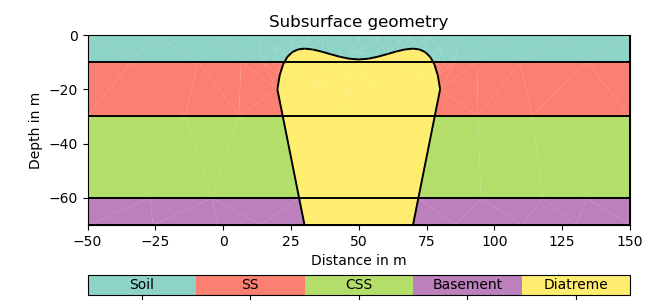
\includegraphics[width=0.6\textwidth]{Figures/Model.png}
    \caption[Synthetic model of simplified diatreme structure]{Synthetic model of simplified diatreme structure. SS is referring to the first sandstone layer and CSS refers to a second, more consolidated sandstone layer.}
    \label{figure:synthetic_model}
\end{figure}
\section{Methods}\label{section:Methods}

\subsection{Mesh generation}\label{section:Mesh}
To discretize the 2D subsurface geometry, especially the diatreme structure, as good as possible an unstructured, triangular mesh is used. This is done in PyGIMLI by using the function \textit{pygimli.meshtools.createMesh()} which is calling the two-dimensional quality mesh generator and Delaunay triangulator \textit{Triangle} \citep{shewchuk1996triangle}. The resulting mesh is shown inf Figure \ref{figure:mesh} and consists mainly of triangles without small and large angles and is therefore suitable for finite element calculations. The big benefit of the unstructured mesh is that it can discretize curved or irregular boundaries better than a rectangular grid and therefore ensures a better accuracy when running calculations on the model. A discretization of the diatreme structure with a rectangular grid would result in steps at the boundaries, rectangular grids were not considered.

Different material properties, i.e. seismic P-wave velocity, electrical resistivity and density, are assigned to the  different geologic formations that are indicated in Figure \ref{figure:synthetic_model}. The values are based on previous geophysical studies of the area as for example \citet{NiklasPlumpe.2015,TimGilberti.2020} and further literature like \citet{geldart2004problems,palacky1988resistivity} and summarized in table \ref{table:properties}. The upper sandstone layer (SS) is assumed to be part of the groundwater aquifer and therefore has a much lower resistivity than the more consolidated and dense sandstone layer below (CSS). This model will be used as an input for the gravimetric, ERT and traveltime tomography forward calculations which are presented in the following sections.

\begin{table}[]
\caption{Material properties of different geologic formations.}
\centering
\begin{tabular}{lccc}
%{m{15mm} m{70mm} m{18mm}}
\hline 
\textbf{Formation} & \textbf{P-wave Velocity}  & \textbf{Electrical Resistivit}  & \textbf{Density}  \\
& \textbf{[$m/s$]}  & \textbf{[$\Omega m$]}  & \textbf{[$kg/m^3$]}\\ \hline 
Soil & $650$ & $120$ & $1250$\\
SS & $3000$ & $1200$ & $2400$\\
CSS & $3600$ & $3500$ & $2500$\\
Basement & $4500$ & $10^8$ & $2650$\\
Diatreme & $2000$ & $10^5$ & $2100$\\
 \hline 
\end{tabular}
\label{table:properties}
\end{table}


\begin{figure}[]
  \centering
  \begin{minipage}[b]{0.48\textwidth}
    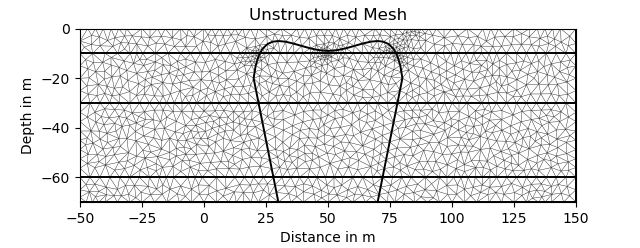
\includegraphics[width=\textwidth]{Figures/Mesh.png}
    \caption[Unstructured mesh]{Unstructured, triangular mesh used to discretize the subsurface geometry.}
    \label{figure:mesh}
  \end{minipage}
  \hfill
  \begin{minipage}[b]{0.48\textwidth}
    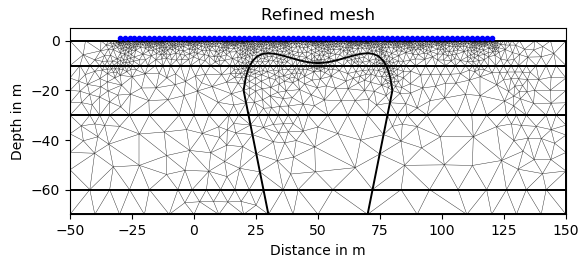
\includegraphics[width=\textwidth]{Figures/ERT_refined_mesh.png}
    \caption[Refined mesh used for ERT calculations]{Refined mesh used for ERT calculations. Here electrodes are between -20 and 120m.}
    \label{figure:refined_mesh}
  \end{minipage}
\end{figure}

\subsection{Electrical Resistivity Tomography}\label{section:ERT}
The ERT method is sensitive to electrical resistivity contrasts in the subsurface due to for example changes in clay content, porosity, pore fluid or ore minerals. First a direct current is inserted into the ground using two electrodes and then the potential difference between two points is measured with two additional electrodes. The electric potential $U$ can be calculated using the Poisson equation: 
\begin{equation}
    \nabla[\sigma (\textbf{r}) \nabla U(\textbf{r})] = -\nabla J
    \label{Eq:poisson}
\end{equation}

Here $\textbf{r}$ stands for the location, $J$ for the injected electrical current, and $\sigma$ for the electrical conductivity which is the inverse of the electrical resistivity $\rho$. This equation builds the basis for the ERT forward calculation \citep{johnson2015accurate}. For a known conductivity distribution, a known injected current and appropriate boundary conditions at the model boundaries, the potential at every location inside the model can be calculated. 

In PyGIMLI the calculation is performed using the module \textit{pygimli.physics.ert} which makes use of the open-source library BERT \citep{gunther20063, rucker20063}. It assumes a Neumann boundary condition (fixed derivation of the potential) for the upper boundary as its is representing the free surface boundary of the Earth. For the remaining boundaries a mixed boundary condition is implemented to avoid unpyhsical field distortions and ensure accuracy of the simulation. 
Using information defined in ert.scheme a finite element simulation can be run to determine the electrical potential in the modelling domain. To ensure numerical accuracy a refinement of the mesh is performed close to the current injection locations as well as the potential measurement locations. The refined mesh is shown in Figure \ref{figure:refined_mesh}. Note that the new mesh has smaller cells close to the surface where the virtual electrodes are located and bigger cells in greater depth. That is done to ensure higher accuracy close to injection points which is crucial for the whole simulation.

Using the results of the simulations the potential differences between two virtual electrodes for two virtual injecting electrodes can be calculated. This can be converted to apparent resistivity $rho_{app}$ according to \citet{kearey2002introduction} as follows:
\begin{equation}
    \rho_{app} = \frac{2\pi}{\frac{1}{\overline{AM}}-\frac{1}{\overline{AN}}-\frac{1}{\overline{BM}}+\frac{1}{\overline{BN}}} \frac{\Delta U}{I} = K \frac{\Delta U}{I}
    \label{Eq:rho_app}
\end{equation}

$\Delta U$ represents the potential difference between the two measurement locations $M$ and $N$, $I$ stands for the strength of the injected electrical current between the locations $A$ and $B$. The distance between an injection point and a measurement point is represented for example by $\overline{AM}$. The factor related to the acquisition geometry is called $K$ and is also often referred to as geometrical factor. To create a more realistic data set, noise is added to the data inside the \textit{simulate()} function. The noise is random and is defined by an absolute value as well as a noise level. The noise level is given in percent and defines the relative noise magnitude on a data point. The absolute noise on the other hand defines a noise magnitude independent from the data point and is therefore defined in the unity of volt $V$. For each data point the bigger of those noise criteria is chosen to define the noise that is contaminating the data.

After generating the synthetic data as described above an inversion is performed in order to turn the apparent resistivity section into a true resistivity distribution. This is done in PyGIMLI via the function \textit{pygimli.frameworks.methodManager.invert()}. This function requires the generated synthetic data as input as well as parameters for the inversion mesh generation and the inversion. The function is starting the inversion process by constructing an inversion mesh based on the acquisition geometry and the additional parameters given as an input. The inverse problem is subject to a non-linear optimization problem as the misfit function $\chi$ needs to be minimized. The misfit criterion $\chi$ is calculated using the synthetic data and the predicted data. A value of approximately $\chi=1$ is desirable as it represents a model that explains the data within the uncertainties. Using a Gauss-Newton algorithm a error-weighted, smoothness-constraint least-squares solution to the inverse problem is determined which can be visualized as a true resistivity distribution. The smoothness constraint is mainly defined through the regularization parameter $\lambda$ which weights between the data fit $\chi$ and the model smoothness. The higher the $\lambda$ value the smoother is the resulting model, however, it results in a worse data fit \citep{Ruecker2017}.

\subsection{Traveltime Tomography}\label{section:TT}
Traveltime tomography, also often referred to as seismic refraction tomography, is a method that is based on seismic refraction in the subsurface. Refracted waves can be observed if a seismic velocity increase can be observed with increasing depth. In that case the wave is travelling faster inside the deeper refractor in comparison with the direct wave which is travelling along the surface such that at a certain distance the refracted wave is overtaking the direct wave. Then the first arrival in the seismic measurements is contributed by the refracted wave \citep{kearey2002introduction}. Synthetic traveltime tomography data is created using the standard routine in the module \textit{pygimli.physics.traveltime}, starting with the setup of the acquisition geometry. Then, a refined mesh is constructed similar to the ERT calculations described in section \ref{section:ERT}. The synthetic data is then generated via the function \textit{pygimli.physics.traveltime.TravelTimeManager.simulate()} which computes the ray paths between sources and sensors. With known ray paths the synthetic data, i.e. the traveltimes, can be calculated according to \citet{zelt2021traveltime} as:
\begin{equation}
    t_i = \sum_j l_{ij}sj
    \label{Eq:TT}
\end{equation}

$t_i$ is the i-th taveltime observation, $l_{ij}$ the length of the i-th ray path segment (corresponding to the i-th observation) in the j-th model cell and $s_j$ is the slowness of the j-th model cell. Note that the slowness $s$ is the reciprocal of the velocity $v$. Noise can be defined similar as it was already described for the synthetic ERT data. Important to mention is that the absolute noise is defined in seconds ($s$) as traveltimes are generated.

After generating the synthetic traveltimes, an inversion of the data is performed similar to the ERT data inversion described in section \ref{section:ERT}. PyGIMLI performs an inversion of the traveltime data by calling the function \textit{pygimli.physics.traveltime.TravelTimeManager.invert()}. The result is, similar to the ERT inversion, an error-weighted, smoothness-constraint least-squares solution in form of a velocity model that explains the data within the uncertainties \citep{Ruecker2017}.


\subsection{Gravimetry}\label{section:Gravimetry}
The gravity method is based on Newton's Law of Gravitation which relates the force $F$ between two bodies with their masses $m_1$ and $m_2$ and the distance $r$ between them as:
\begin{equation}
    F = \frac{Gm_1 m_2}{r^2}
    \label{Eq:Newton1}
\end{equation}

The constant $G$ is called the gravitational constant and holds a value of $6.67*10^{-11}m^{3}kg^{-1}s^{-2}$. Assuming that one body is the Earth with a mass $M$ and a radius $R$, the gravitational force on an object on the Earth surface would be:
\begin{equation}
    F = \frac{GM}{R^2}m = gm
    \label{Eq:Newton2}
\end{equation}

As shown in the equation \ref{Eq:Newton2} the gravitational force on a body is a product of the gravitational acceleration $g$, often also referred to as gravity, and its mass. In gravimetry it is most useful to describe the gravitational field in form of its potential $U$ as the gravitational acceleration is the gradient of the potential $U$. The magnitude of the potential depends on the radius as well as on the density distribution in the subsurface and therefore measurements of the gravitational acceleration can be used to gain knowledge of subsurface structures \citep{kearey2002introduction}.

A synthetic gravity study of the simplified diatreme model is performed in PyGIMLI. This is achieved by applying the function \textit{pygimli.physics.gravimetry.solveGravimetry()} to the mesh with a defined sensor geometry and density distribution. The forward calculation of the gravimetric potential is the performed after \citet{won1987computing}. The synthetic data then shows then the gravitational response of the density distribution. To isolate the gravity response of the anomaly synthetic data of the layered subsurface without the diatreme structure will be generated and deducted from the first simulation data. The resulting data shows the effect of the diatreme structure on the gravitational acceleration, i.e. the first derivative of the gravitational potential. As PyGIMLI does not offer a fast and easy way yet to invert gravity data in 2D and due to the lack of time during the research module, the synthetic gravity data is not inverted in this work. However, the synthetic data will be visualized and discussed.


\section{Results}\label{section:Results}

A summary of all settings used for the forward and inverse calculations is presented in tables \ref{table:settings_forw} and \ref{table:settings_inv}. In the following subsections a reasoning for these parameters will be presented and results will be shown. 

\subsection{Electrical Resistivity Tomography}
For the ERT data generation 76 synthetic electrodes over a distance of 140m are used to simulate the potential differences. These values are chosen as the represent a realistic field setup as it could be done as part of a thesis work. The same reasoning is also used for the other methods. Three different electrode configurations are simulated, namely the Dipole-Dipole, Schlumberger and Wenner configuration. The noise level is defined with 2.5\% and the absolute value of 0.001mV. As the absolute noise is set very low, the data is contaminated by the relative noise magnitude. The resulting data can be visualized in terms of apparent resistivity in a pseudo section. This is shown in Figure \ref{figure:ERT_inversion_misfits} in the top row. Since no topography is considered the pseudo section already show a strong subsurface anomaly as the apparent resistivities are varying between 100$\Omega m$ and 1000$\Omega m$. We can also see that the Dipole-Dipole configuration is generating the most data points as it shows the most cells in the section. 

Using the respective inversion parameters which are stated in table \ref{table:settings_inv}. The setting for the inversion were found by trial and assumed to be good as the data misfit value $\chi$ is close to 1 for all three configurations. A data misfit of approximately 1 indicates a good data fit and is therefore desirable. The resulting true resistivity sections are presented in Figure \ref{figure:ERT_inversion_comp}. It can be seen that all three configurations do not hold significant information below a depth of 40m. They show a strong high-resistivity anomaly in the centre of the section at a depth between approximately 10m and 30m that is reaching resistivities over 10000 $\Omega m$. A shallow very conductive layer is shown up to a depth of around 10m. Left and right of the strong resistive anomaly and below the conductive top layer another unit with resistivities of around 1000-2700$\Omega m$ can be identified. Important to mention is that the Dipole-Dipole result appears to show slightly higher resistivity values below the conductive top layer but this is produced by the plotting as the Dipole-Dipole configuration has more measurements resulting in a higher coverage and therefore less transparent model cells. A more detailed discussion of the final inversion results of the different ERT configurations is presented in section \ref{section:Discussion}.

\begin{figure}[H]
  \centering
    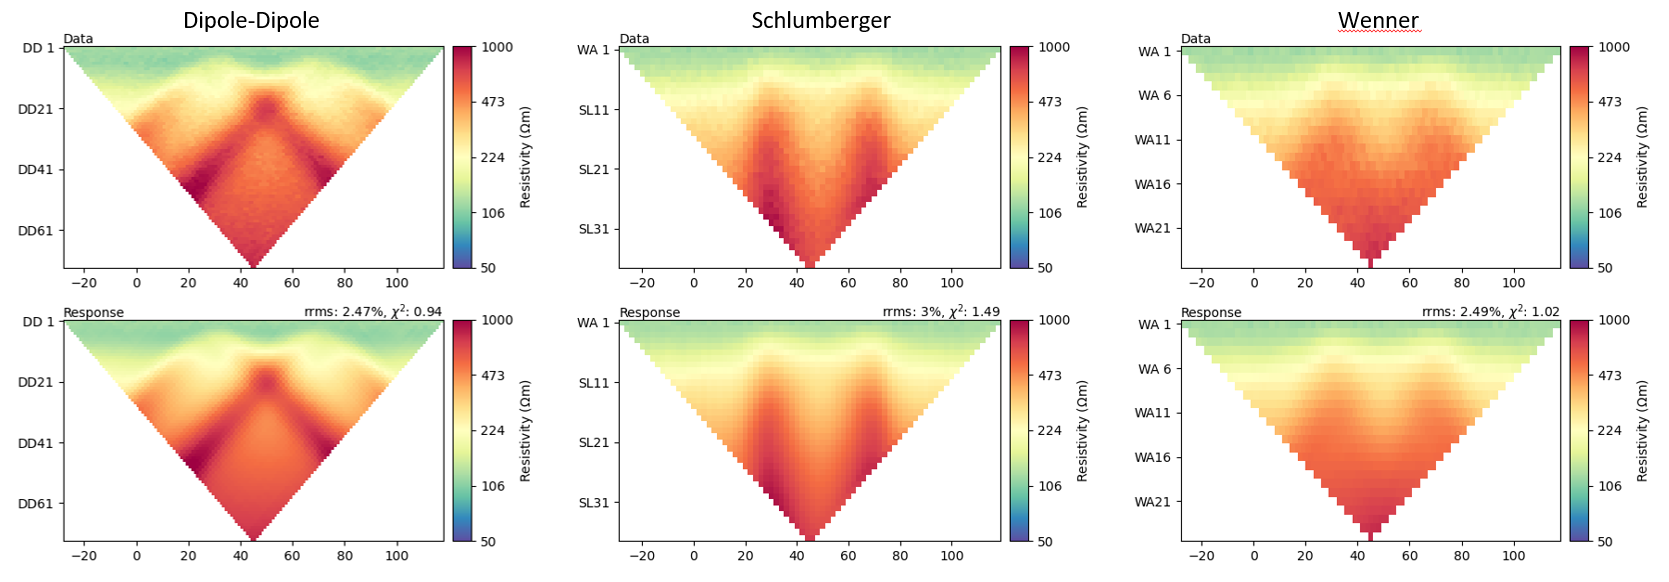
\includegraphics[width=\textwidth]{Figures/ERT_inversion_overview.png}
    \caption[ERT inversion result misfit]{Inversion result misfit of the Dipole-Dipole (left), Schlumberger (middle) and Wenner electrode configuration. At the top the synthetic data pseudo section is shown and below the pseudo section resulting from the inversion is presented. On top of the inverse model response the root mean square error (RMS) and the data misfit $\chi$ is stated.}
    \label{figure:ERT_inversion_misfits}
\end{figure}

\begin{figure}[H]
  \centering
    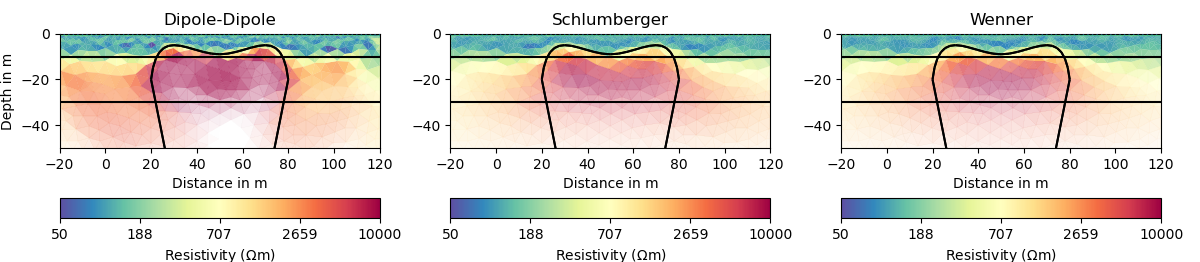
\includegraphics[width=\textwidth]{Figures/ERT_Inv_comp.png}
    \caption[Final resistivity models after inversion]{Final ERT inversion results. The results of the Dipole-Dipole (left), Schlumberger (middle) and Wenner configuration (right) are superimposed by the subsurface geometry used for synthetic data generation. The transparency of the mesh cells indicates the data coverage as opaque cells represent higher data coverage.}
    \label{figure:ERT_inversion_comp}
\end{figure}

\subsection{Traveltime Tomography}\label{section:Res_TT}

For the traveltime tomography data generation 91 sensors with a spacing of 2m are defined between -40m and 140m. Every third sensor location is chosen to be a shot location, resulting in 31 shots. Just as the synthetic ERT data, noise is produced and added to the generated data. For the traveltime tomography the absolute noise is set to 1ms and the relative noise to 0.01\%. This means that for early arrivals, i.e. small source-receiver offsets, the absolute noise is defining the noise magnitude while for later arrivals, i.e. large offsets, the relative noise parameter is the deciding factor. The synthetic data is presented in the left part of Figure \ref{figure:TT_inversion_misfits}. In the data matrix, the zero offset measurements, i.e. measurements with an identical source and receiver location, are excluded and appear white. The simulated traveltimes are directly converted to apparent velocities using the source receiver distance.

The inversion of the traveltimes results in an estimated data matrix which is shown in the right part of Figure \ref{figure:TT_inversion_misfits}. As seen, the data misfit is very close to one and therefore a suitable inversion result can be assumed. Figure \ref{figure:TT_inversion_comp} presents the resulting velocity model on the left and the corresponding ray coverage on the right. As seen in the right plot, the data does not hold any information about the subsurface below 30m depth as well as close to the left and right model boundary. Therefore, the model values in these regions are not reliable as they are not data driven but purely depending on the initial model of the iterative inversion scheme. Note that this part of the model space will not be discussed further as it does not contribute to the objectives of this synthetic data study. In the upper 10m of the model we find a low-velocity layer which holds velocities below 1000m/s. Between -20m and 20m and well as between 80m and 120m at a depth of 10m to 30m, high-velocity structures appear with velocities of 3000-3500m/s. In between those high-velocity anomalies two velocity anomalies with around 1500m/s (at a distance of 20-40m and 60-80m). Between 40m and 60m a structure with approximately 2900m/s can be observed. Further discussion of the results and a comparison with the other methods is done in section \ref{section:Discussion}.

\begin{figure}[]
  \centering
    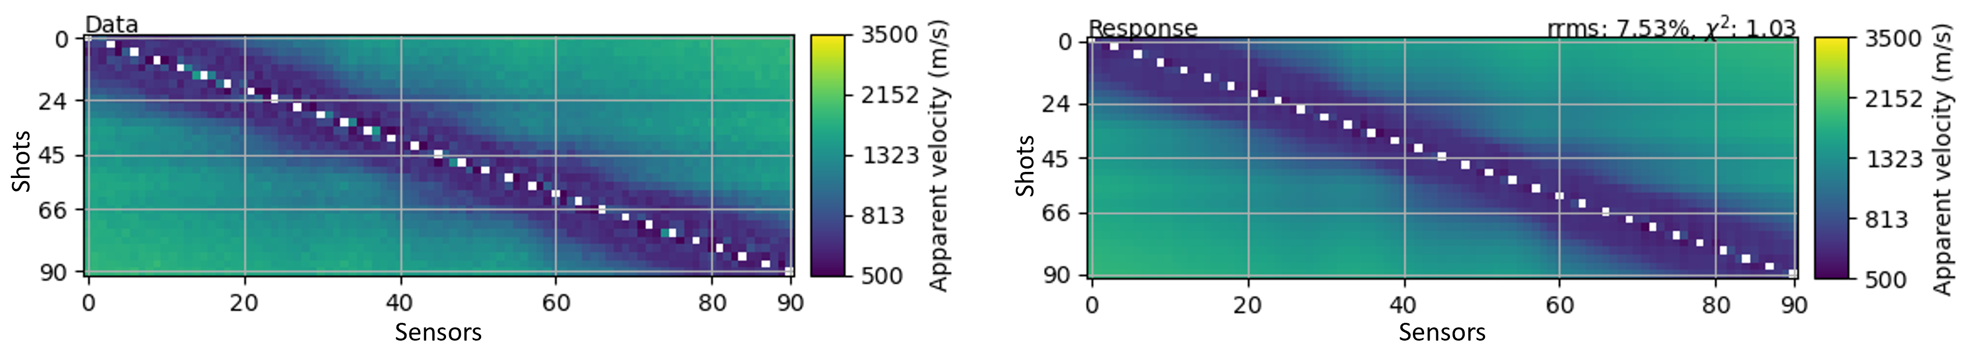
\includegraphics[width=\textwidth]{Figures/TT_RF_labels.png}
    \caption[Traveltime inversion result misfit]{Inversion result misfit of the synthetic traveltime tomography data. On the left the synthetic data is shown and on the right the estimated data resulting from the inversion is presented. On top of the inverse model response the root mean square error (RMS) and the data misfit $chi$ is stated.}
    \label{figure:TT_inversion_misfits}
\end{figure}


\begin{figure}[]
  \centering
    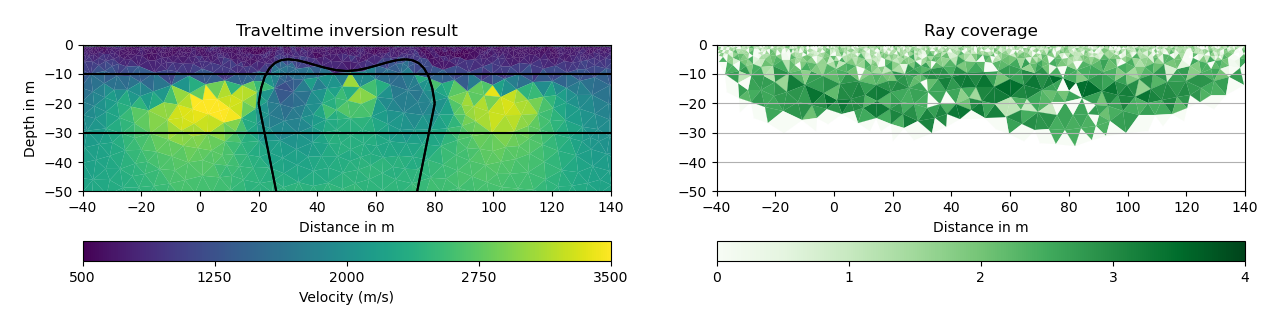
\includegraphics[width=\textwidth]{Figures/TT_comp.png}
    \caption[Final velocity model after inversion]{Final traveltime inversion results. The final velocity model (left) is superimposed by the subsurface geometry used for synthetic data generation. The ray coverage of the traveltime tomography is shown on the right.}
    \label{figure:TT_inversion_comp}
\end{figure}

\subsection{Gravimetry}
According to table \ref{table:settings_forw} the synthetic gravity data was generated using a 140m long spread of 71 stations. As no inversion is performed on these synthetic data set, no noise is generated and superimposed on the data. The synthetic gravity measurements can be seen in Figure \ref{figure:grav}. As the parameter table \ref{table:properties} states, the diatreme has a lower density than the surrounding dense sandstone and therefore also produces a negative gravity response in the synthetic data. Due to the irregular upper boundary of the diatreme structure two saddle points in the gravity anomaly can be observed at 30m and 70m. Figure \ref{figure:grav} also shows that the anomaly reaches its maximum magnitude of approximately -0.3mGal at a distance of 50m which coincides with the center axis of the diatreme structure.

\begin{figure}[]
  \centering
    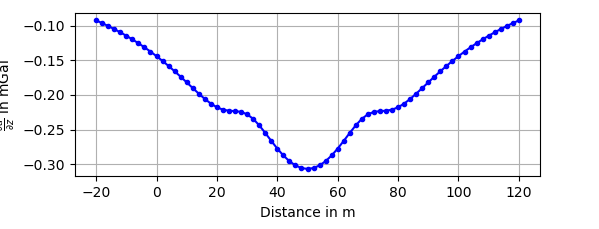
\includegraphics[width=0.8\textwidth]{Figures/GRVA_dataonly.png}
    \caption[Synthetic gravity data]{Synthetic gravity data points.}
    \label{figure:grav}
\end{figure}



\section{Discussion}\label{section:Discussion}
+ comment on differences between ert configs
+ comment on TT result
+ comment comment  on what method resolves what parts
+ include gravimetric data 

+ conclusion for master thesis
\section{Conclusion}\label{section:Conclusion}



%%% Bibliography
\newpage
\printbibliography
\newpage


%%%%%%%%%%%%%%%%%%%%%%%%%%%%%%%%%%%%%%%%%%%%%%%%%%%%%
%%% Appendix
\newpage
\appendix
\section{Appendix}
\setcounter{figure}{0}
\setcounter{table}{0}
\renewcommand{\thetable}{A\arabic{table}}
\counterwithin{figure}{section}

\subsection{Settings for forward and inverse computations}\label{appendix:Settings}

\begin{table}[H]
\centering
\caption{Settings for forward computations.}
\begin{tabular}{llc}
\hline
\textbf{Method}       & \textbf{Parameter}   & \textbf{Value} \\ \cline{1-3}
ERT                   & first electrode      & -30 m\\
                      & last electrode       & 120 m\\
                      & number of electrodes & 76\\
                      & noise level          & 2.5 \% \\
                      & absolute noise       & 0.001 mV \\ \cline{1-3}
Traveltime Tomography & first sensor         & -40 m \\
                      & last sensor          & 140 m \\
                      & number of sensors    & 91\\
                      & shot spacing         & 6 m\\
                      & noise level          & 0.01 \%  \\
                      & absolute noise       & 1 ms \\ \cline{1-3}
Gravity               & first sensor         & -20 m  \\
                      & last sensor          & 120 m   \\
                      & number of sensors    & 71       \\ \cline{1-3}
\end{tabular}
\label{table:settings_forw}
\end{table}

\begin{table}[H]
\centering
\caption{Settings for inversions.}
\begin{tabular}{lcccc}
\hline
Parameter       & ERT - DD & ERT - SLM & ERT - WA & Traveltime Tomography \\ \hline
secNodes        & 2                   & 2                  & 2            & 2                     \\
paraMaxCellSize & 20                  & 20                 & 20           & 20                    \\
lam             & 3                   & 17                 & 17           & 2.5                    \\
zWeight         & 0.3                 & 0.2                & 0.3          & -                     \\
vTop            & -                   & -                  & -            & 600                   \\
vBottom         & -                   & -                  & -            & 2700                  \\ \hline
\end{tabular}
\label{table:settings_inv}
\end{table}
\newpage
\subsection{Data management}\label{section:Data_management}

\paragraph*{Software}
Data processing, inversions and modelling will be performed in open-source packages in Python (e.g. PyGIMLI, Numpy etc.). It is possible that SeismicUnix or Reflexw will be used for seismic data inspection.

\paragraph*{Inputs}
Input data for the Master thesis research will be previously acquired field data. A summary of the different data is shown in table \ref{table:Input_data}. As the data was acquired as part of previous thesis works at the Ruhr-Universität Bochum and not published yet, thos files will be stored in a final repository which will be made available for the supervisors. This will possibly be done via Sciebo. This will be done as well with additional data that might be acquired as part of this thesis work.

\begin{table}[!htb]
\caption{Overview of input data.}
\centering
\begin{tabular}{lcc}
%{m{15mm} m{70mm} m{18mm}}
\hline 
\textbf{Method} & \textbf{Year} & \textbf{Size}  \\ \hline 
Magnetics & 2011 & 1.6 MB\\
& 2012 & 212 KB\\
ERT & 2015 & 158 MB\\
& 2020 & 128 KB\\
Seismics & 2015 & 683 MB\\
& 2017 & 656 MB\\
Photogrammetry & 2020 & 12 GB\\
& & \textbf{Total:} 14 GB\\
 \hline 
\end{tabular}
\label{table:Input_data}
\end{table}

\paragraph*{Outputs}outputs: Formats, data size, where stored
Intermediate and final results of the thesis work include processed data, inversion results in form of models, Python scripts and Figures generated to visualize results. Those will be stored in a Github repository which will be made available for the supervisors. For the time of the research this repository will be kept private. However, after finishing the thesis work the repository might be made public depending on the outcome of the thesis work. Also, the report in form of .tex and other \LaTeX-formats will be stored in the repository to ensure version control of the writing process. It also makes an easy access and commenting for the supervisors possible.

%\chapter{More Pics}\label{appendix:B}
This appendix includes additional pics

\section{Pic 1}
\begin{figure}[H]
\noindent
\includegraphics[width=0.7\textwidth]{Titlepage_files/RWTH_AICES_logo.png}
\caption[Logo AICES]{RWTH Aachen Logo of AICES group.}
\label{figure:aices}
\end{figure}

\section{Pic 2}
\begin{figure}[H]
\noindent
\includegraphics[width=0.7\textwidth]{Titlepage_files/RWTH_CGGR_logo.png}
\caption[Logo CGGR]{RWTH Aachen Logo of CGGR group.}
\label{figure:cggr}
\end{figure}

\section{Pic 3}
\begin{figure}[H]
\noindent
\includegraphics[width=0.7\textwidth]{Titlepage_files/RWTH_EONERC_logo.png}
\caption[Logo EONRC]{RWTH Aachen Logo of EON Research center.}
\label{figure:eonrc}
\end{figure}
%\input{appendix/appendix-c}


%Include document printout
%\verbatiminput{XXX}

\end{document}